\documentclass{article}
\usepackage{tikz}

\begin{document}

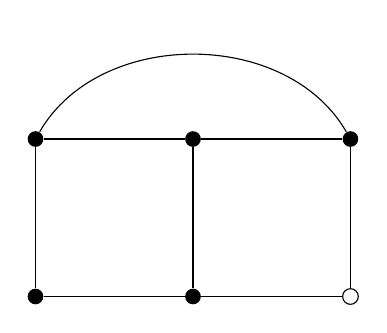
\begin{tikzpicture}[scale=1]
    % Define the nodes
    \node (a) at (0,0) [circle,fill,inner sep=2pt] {};
    \node (b) at (2,0) [circle,fill,inner sep=2pt] {};
    \node (c) at (4,0) [circle,fill,inner sep=2pt] {};
    \node (d) at (2,-2) [circle,fill,inner sep=2pt] {};
    \node (e) at (0,-2) [circle,fill,inner sep=2pt] {};
    \node (f) at (4,-2) [circle,draw,inner sep=2pt] {};

    % Draw the edges
    \draw (a) -- (b);
    \draw (b) -- (c);
    \draw (a) -- (e);
    \draw (b) -- (d);
    \draw (c) -- (f);
    \draw (d) -- (e);
    \draw (e) -- (f);
    \draw (a) to[bend left=60] (c);
\end{tikzpicture}

\end{document}